\documentclass{standalone}
\usepackage{tikz}
\usepackage{ctex,siunitx}
\usepackage{tkz-euclide}
\usepackage{amsmath}
\usepackage{chemmacros,siunitx}
\usetikzlibrary{patterns, calc}
\usetikzlibrary {decorations.pathmorphing, decorations.pathreplacing, decorations.shapes,}
\begin{document}
\Large
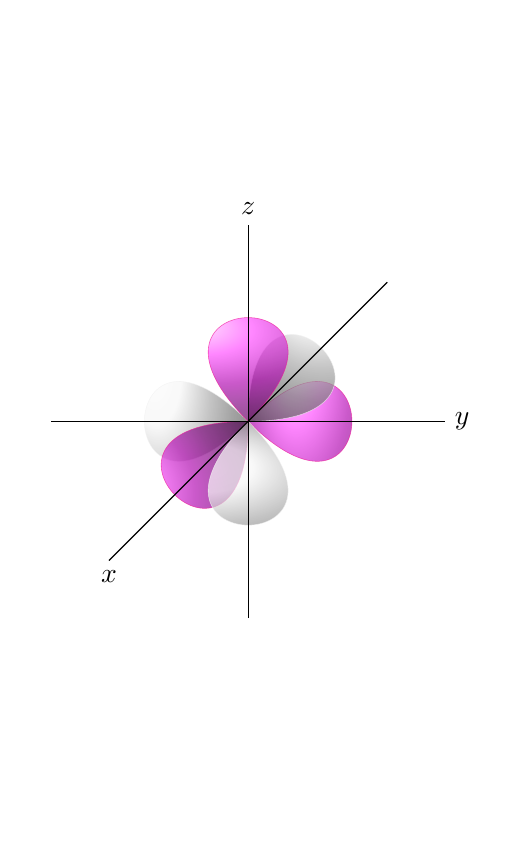
\begin{tikzpicture}
  \useasboundingbox(-2.8,5)rectangle(3.2,-5);
  \node [opacity=0.7]{\orbital[angle=0,scale=2.5,color=magenta]{p}};
  \node [opacity=0.7]{\orbital[angle=225,scale=2.5,color=magenta]{p}};
  \node [opacity=0.7]{\orbital[angle=90,scale=2.5,color=magenta]{p}};
  \draw(225:2.5)node[below]{$x$}--(45:2.5);
  \draw(0,-2.5)--(0,2.5)node[above]{$z$};
  \draw(-2.5,0)--(2.5,0)node[right]{$y$};
\end{tikzpicture}
\end{document}